

Pour l'estimation des distance on doit décomposer l'espace en plusieurs dimensions. Pour simplifier on va diviser l'espace en 2 dimensions.

Pour 2 têtes, On prend comme référence le plan qui passe par ces 2 têtes et dont une des 2 dimensions est parrallêle au sol (donc au bord inférieur de l'image). Ainsi on a les 2 dimensions:

\begin{itemize}
    \item la dimension X est la dimension parrallêle au bord inférieur de l'image
    \item la dimension Y est celle perpendiculaire à celle-ci, mais qui suit le plan passant par les 2 têtes.
\end{itemize}


Ainsi, en obtenant la projection de lu vecteur disctantce sur ces 2 dimensions, on calcul la distance totale avec le théorème de pythagore.

Par ailleurs on notera : $(x_1, y_1)$ et $(x_2, y_2) $les coordonnées des 2 têtes (en pixel), $(d_1,d_2)$ leur profondeur respective (en mêtre) et $(dX, dY)$ le vecteur distance entre les 2 têtes (en mêtres). Et $f$ la focale de la caméra (en pixel).

\subsection{distance sur l'axe Y}

Pour calculer la distance sur l'axe y, qui est en fait la différence de profondeur corrigé pour prendre en compte la position relative des personnes, on utilise le théorème d'alkachy.

\begin{figure}[h!]
    \centering
    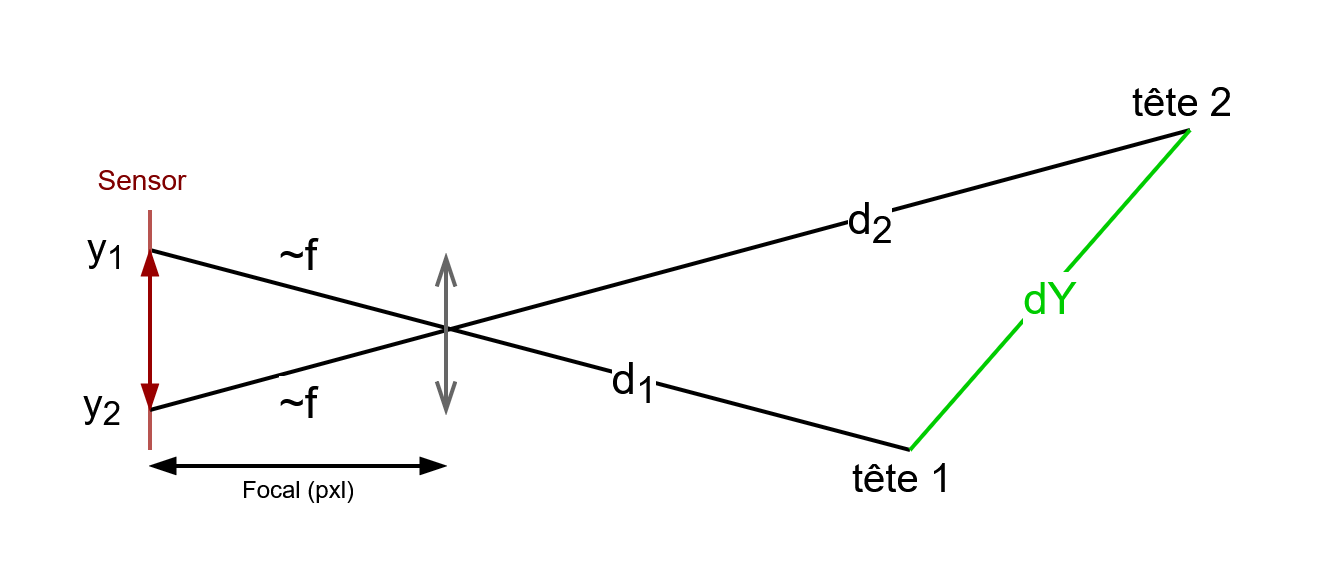
\includegraphics[width=0.45\textwidth]{images/dY_estimation.drawio.png}
    \caption{Modélisation pour la distance sur l'axe Y.}
    \label{fig:alkachy}
\end{figure}

\begin{equation}
    dY^2 = d_1^2 + d_2^2 - 2d_1d_2 ( 1 - ( \frac{|y_2-y_1|^2}{2*focal^2} ) )
\end{equation}

\subsection{distance sur l'axe X}

Pour la calculer la distance dans cette dimensions c'est assez facile, en utilisant la formume \ref{eq:camera-relation} on détermine la distance en mêtre au niveau de x1 avec d1, puis au niveau de x2 avec d2.
On fait l'hypothèse que la perspecive est parfaitement plongeante ce qui fait qu'il faut enlever la moitié de la différence pour obtenir la distance entre les 2 têtes (avec $d_2>d_1$).

\begin{align}
    dX1 &= (x_2-x_1) * d1 / focal \\
    dX2 &= (x_2-x_1) * d2 / focal \\
    dX  &= dX2 - (dX2-dX1)/2 \\
        &= (dX2 + dX1) /2
\end{align}

\subsection{distance totale}

Ainsi, on obtiens grâce au théorème de pythagore on peut calculer la distance inter-personnes en mètre.

\begin{figure}[h!]
    \centering
    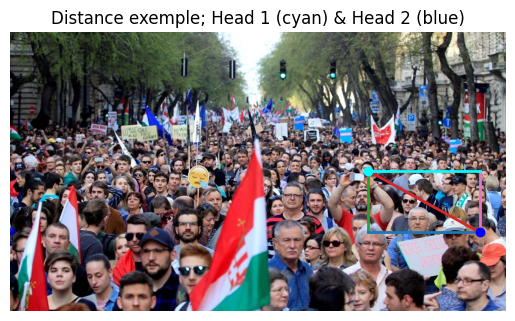
\includegraphics[width=0.45\textwidth]{images/exemple_dist_estimation.png}
    \caption{Exemple de distance estimé entre 2 têtes.}
    \label{fig:distance-estimation}
\end{figure}

Par exemple, sur notre exemple entre les 2 têtes de la Figure \ref{fig:distance-estimation}, on obtient les distances:

\begin{itemize}
    \item $d_1  = 20.82 m \text{ (point cyan)}$
    \item $d_2  = 10.9 m \text{ (point bleu)}$
    \item $dY  = 9.93 m \text{ (vert)}$
    \item $dX  = 1.12 m$
    \item $d_{total} = 10.04m \text{ (rouge)}$
\end{itemize}

\section{Pour aller plus loin}

Grâce aux estimations de distances entre les têtes, on peut envisager plusieurs applications direct:

\begin{itemize}
    \item Soit construire un graphe de distance estimé entre les personnes dans le plan du sol.
    \item Soit placer directement les tête dans un espace 3D en utilisant les vecteurs de distance estimé, ce qui sera certainement plus précis 
\end{itemize}

Dans tous les cas ces mesures nous permettent d'estimer la densité de personnes dans une foule avec une simple caméra, et donc évaluer les risques associés ou simplement retracer les mouvements des personnes au cours du temps.

\section{Conclusion}

En conclusion, nous avons utilisé des modèles de deep learning avancés pour concevoir une application hybride efficace. Cette solution fusionne détection de têtes et estimation de profondeur, offrant des résultats satisfaisants.

Notre méthode présente des limites, notamment l’imprécision héritée des modèles combinés, qu’on a tenté de compenser. Une approche "end-to-end" aurait pu être plus précise, mais nous manquions du dataset nécessaire.

Ses atouts reposent sur l’utilisation de modèles pré-entraînés performants, demandant peu de ressources. Cela la rend idéale pour notre projet et facilement adaptable aux progrès futurs.

Enfin, il nous manque une évaluation chiffrée pour juger pleinement notre méthode. Une expérience réelle avec caméra ou une simulation via un moteur de jeu vidéo pourrait serait la prochaine étape pour valider nos performances.
